\documentclass[11pt,ngerman,a4paper]{article}
%Gummi|061|=)
\usepackage{amsmath}
\usepackage{a4wide}
\usepackage{url}
\usepackage{amsthm}
\usepackage{amsbsy}
\usepackage{amssymb}
\usepackage{inputenc}
\usepackage{rotating} 
\usepackage{here}
\usepackage{graphicx}
\usepackage{paralist}
\usepackage{selinput}
\usepackage[separate-uncertainty=true]{siunitx}
\usepackage{booktabs}
\sisetup{}
\SelectInputMappings{%
adieresis={ä},
germandbls={ß},
}
\title{\textbf{Versuch US1: Grundlagen der Ultraschalltechnik}}
\author{Martin Bieker\\
		Julian Surmann\\
		\\
		Durchgef\"{u}hrt am 22.04.2014\\
		TU Dortmund}
\date{}
\usepackage{graphicx}
\begin{document}
\renewcommand\tablename{Tabelle}
\renewcommand\figurename{Abbildung}
\maketitle
\thispagestyle{empty}
\newpage
\clearpage
\setcounter{page}{1}


\section{Einleitung}
Ultraschall wird in vielen Bereichen der Medizin und Technik als bildgebendes Verfahren und zur zerst\"orungsfreien Werkstoffuntersuchung eingesetzt. In diesem Versuch sollen die Grundlagen dieser Technik untersucht werden.
\section{Theorie}

Schallwellen im Frequenzbereich von \SI{20}{\hertz} bis \SI{1}{\giga\hertz} werden als Ultraschall bezeichnet. Schallwellen sind Druckschwankungen, welche sich als longitudinale Wellen durch ein Medium ausbreiten. Die Ausbreitungsgeschwindigkeit $c$ h\"angt dabei vom Medium ab, in dem sich die Welle befindet. Propagiert der Schall von einem Medium in ein Anderes treten f\"ur Wellen typische Effekte wie zum Beispiel Brechung und Reflexion auf. Dieses Verhalten an Grenzfl\"achen wird im Rahmen der Ultraschalltechnik zur Untersuchung eines K\"orpers verwendet. 
\subsection{Erzeugung und Detektion von Ultraschall}
In den meisten Anwendungen wird Ultraschall mit Hilfe des reziproken piezo-elektrischen Effektes erzeugt. Hierbei wird ein Kristall (zum Beispiel Quarz) durch ein angelegtes elektrisches Feld zu Schwingungen angeregt. Stimmt die Frequenz der Anregung mit der Eigenfrequenz des Kristalls \"uberein, so kommt es auf Grund von Resonanz zu einer Abstrahlung von Ultraschallwellen mit hoher Intensit\"at.  Die Umkehrung dieses Effektes wird auch zur Detektion des reflektierten Ultraschalls angewandt.
\subsection{Messverfahren} 
Die Messung kann entweder mit einer oder mit zwei Ultraschallsonden durchgef\"uhrt werden. Letzteres ist das so genannte Durchschallungssverfahren. Hierbei wird der von einem Empf\"anger erzeugte Ultraschall durch die Probe geschickt und von einem Empf\"anger aufgezeichnet. Unregelm\"assigkeiten zeigen sich durch eine geringere Intensit\"at am Detektor. Um diese Fehlstellen zu lokalisieren wird das Impuls-Echo-Verfahren verwendet. Hier dient eine Sonde sowohl als Empf\"anger und als Sender. Diese sendet einen Ultraschallimpuls aus und misst danach die reflektierten Amplitude sowie deren Laufzeit. Diese Werte k\"onnen auf verschiedene Arten dargestellt werden.
\subsection{Darstellung der Messergebnisse}
Es gibt mehrere M\"oglichkeiten, die durch die Laufzeitmessung gewonnenen Daten darzustellen.
\paragraph{A-Scan} Beim so genannten Amplituden-Scan werden die gemessenen Amplituden in einen Diagramm gegen die Laufzeit aufgetragen. So k\"onnen eindimensionale Strukturen untersucht werden. 
\paragraph{B-Scan}
Beim Brightness-Scan wird ein zweidimensionales Schnittbild der untersuchten Struktur erzeugt. Dabei die Sonde gleichm\"assig \"uber das Objekt bewegt und die gemessenen Amplituden in verschiedenen Helligkeitsstufen dargestellt.  
\paragraph{TM-Scan} Beim Time-Motion-Scan werden laufend B-Scans in kurzen Abst\"anden erstellt, um Bewegungen innerhalb des untersuchten Objektes darzustellen.

\section{Durchf\"uhrung }
Die Messungen werden mit einem Messcomputer durchgeführt, an welchen über einen Verstärker verschiedene Ultraschallsonden angeschlossen werden können. Es können \SI{1}{\mega\hertz}, \SI{2}{\mega  \hertz} und \SI{4}{\mega\hertz}-Sonden verwendet werden. Die Messdaten werden dann mit einer speziellen Software auf dem Messcomputer als A-Scan oder B-Scan dargestellt.
\subsection{Messung der Schallgeschwindigkeit in Acryl}
Die Bestimmung der Schallgeschwindikeit durch eine Laufzeitmessung wird an drei zylinderf\"ormigen Proben durchgef\"uhrt. Es muss zuerst die Strecke, welche der Schall in den Proben zur\"ucklegt gemessen werden. Hierzu wird die H\"ohe der Zylinder mit Hilfe einer Schieblehre bestimmt.  
\subsubsection{Impuls-Echo-Verfahren}
Zur Messung der Laufzeit mittels Impuls-Echo-Verfahren wird eine \SI{2}{\mega\hertz} Ultraschall-Sonde an einen der Zylinder gekoppelt. Mit Hilfe eines A-Scans wird die Laufzeit in Abh\"angigkeit von der Zylinderh\"ohe bestimmt. Diese Messungen werden mit einer 1  \SI{}{\mega\hertz} Sonde wiederholt. 
\subsubsection{Durchschallungsverfahren}
Bei dieser Messungen werden jeweils zwei \SI{2}{\mega\hertz} Sonden an die Stirnseiten der Zylinder gekoppelt. Danach wird die Laufzeit des Schalls durch den Zylinder mit einem A-Scan ermittelt. Die Messung wird mit den anderen Zylindern wiederholt.
\subsection{Untersuchung eines Acrylblocks auf Fehlstellen}
\begin{figure}[h]
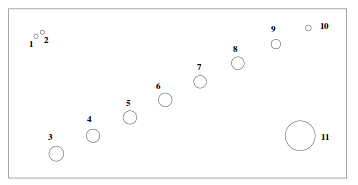
\includegraphics[width=8cm]{quaderbild.png}
\caption{Quader mit Störstellen [1]}
\label{block}
\end{figure}
Abbildung \ref{block} zeigt den zu untersuchenden Acrylblock. Zur Bestimmung von Lage und Groesse der Fehlstellen (Bohrungen) werden zun\"achst die Abmessungen des Blocks mit einer Schieblehre bestimmt. Danach wird eine \SI{1}{\mega\hertz} Sonde auf die Oberseite des Blocks gekoppelt und deren Abstand zu den einzelnen Fehlstellen durch einen A-Scan bestimmt. Dabei sind die im ersten Versuchsteil bestimmten Laufzeitfehler der Sonde zu ber\"ucksichtigen. Um die Groesse der Bohrungen zu bestimmen die Sonde an der entgegengesetzten Seite angekoppelt und der Abstand der Fehlstellen zur Unterseite durch einen weiteren A-Scan bestimmt. Da die Genauigkeit der Sonden von der Frequenz des Ultraschalls abh\"angen kann werden gerade durchgef\"uhrten Messungen mit einer 1 \SI{}{\mega\hertz} Sonde wiederholt. 

\noindent
Danach wird um die Lage und Form der Bohrungen zu bestimmen ein B-Scan durchgef\"uhrt. Hierzu wird die Sonde gleichm\"assig und langsam \"uber den Acrylblock bewegt, damit am Messcomputer ein zweidimensionales Schnittbild erzeugt werden kann.

\subsection{Vermessung eines  Augenmodells}
Im letzten Versuchsteil sollen die Abmessungen eines Augenmodells bestimmt werden. Dazu wird wie in Abbildung \ref{auge} gezeigt, eine \SI{2}{\mega\hertz} Sonde auf die Hornhaut des Modells gekoppelt. Mit einem A-Scan werden die Reflexionen des Ultraschalls an Iris, Linse und Retina bestimmt.
\begin{figure}[h]
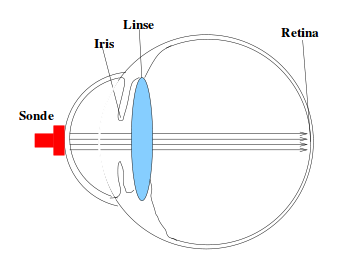
\includegraphics[width=8cm]{augebild.png}
\caption{Modell eines Auges [1]}
\label{auge}
\end{figure}



\section{Auswertung}
\subsection{Bestimmung der Schallgeschwindigkeit mit dem Impuls-Echo-Verfahren}
Die drei Acrylzylinder haben folgende Abmessungen:
 \begin{table}[h]
\centering
 \begin{tabular}{|c||c|c|c|}
 Zylinder & Zylinder 1 & Zylinder 2 & Zylinder 3 \\
  Länge [m] & 0.0397 & 0.0804 & 0.01205 \\
 \end{tabular}
\caption{Maße der Acrylzylinder}
\end{table}
\newline Mit Hilfe der Sonden wurden folgende Laufzeiten des Echos ermittelt (Tabelle 2).
 \begin{table}[h]
\centering
 \begin{tabular}{|c||c|c|c|}
 Zylinder & Zylinder 1 & Zylinder 2 & Zylinder 3 \\
 Laufzeit (2 MHz) [$10^{-6}s$] & 88.7 & 59.7 & 29.9 \\
 Laufzeit (1 MHz) [$10^{-6}s$] & 90  & 60.9 & 31.0 \\
 \end{tabular}
\caption{Laufzeitmessung mit Impuls-Echo-Verfahren}
\end{table}
\newline
Mit Hilfe der Formel $v=\frac{s}{t}$ ergeben sich dann die Schallgeschwindigkeiten (Tabelle 3)
\begin{table}[h]
\centering
 \begin{tabular}{|c||c|c|c|}
 Zylinder & Zylinder 1 & Zylinder 2 & Zylinder 3 \\
 $v_{Schall}$ (2 MHz) [m/s] & 2656 & 2693 & 2717 \\
 $v_{Schall}$ (1 MHz) [m/s] & 2561  & 2640 & 2678 \\
 \end{tabular}
\caption{Schallgeschwindigkeit mit Impuls-Echo-Verfahren}
\end{table}
\newline
Allerdings weisen diese Schallgeschwindigkeiten einen systematischen Fehler auf. Mit Hilfe von linearer Regression wird die Funktion der Zeit in Abhängigkeit von der Strecke aufgetragen. Die Umkehrung der Steigung dieser Funktion ist die eigentliche Schallgeschwindigkeit. Der Laufzeitfehler ist mit dem Y-Achsenschnittpunkt der Funktion gegeben. Die geplotten Regressionsgeraden sind in Abbildung 3 und 4 (Anhang) ersichtlich.

Die Schallgeschwindigkeiten der beiden Messungen ergeben sich damit zu 2739 m/s und 2748 m/s. Der Lautzeitfehler beträgt $2.07056306762*10^{-6} s$ (1 MHz) bzw. $1.06907427036*10^{-6} s$ (2 MHz).
Die Schallgeschwindigkeiten liegen mit einer Abweichung von weniger als 3 \%  an dem in der Literatur angegebenen Wert von 2670 m/s.
\subsection{Bestimmung der Schallgeschwindigkeit mit dem Durchschallungs-Verfahren}

Die Abmessungen der Acrylzylinder sind Abschnitt 4.1 zu entnehmen. Die errechneten Werte der Schallgeschwindigkeit in Acryl sind in Tabelle 4 zu erkennen.
\begin{table}[h]
\centering
 \begin{tabular}{|c||c|c|c|}
 Zylinder & Zylinder 1 & Zylinder 2 & Zylinder 3 \\
 $v_{Schall}$ (2 MHz) [m/s] & 2496 & 2619 & 2672 \\
 \end{tabular}
\caption{Schallgeschwindigkeit mit Durchschallungsverfahren}
\end{table}
\subsection{Untersuchung eines Acrylblocks auf Fehlstellen}
Der zu untersuchende Acrylblock ist 0.08 m hoch, 0.15 m breit und 0.042 m tief. Die Messungen finden über die Strecke von 0.08 m statt. Aus der Wellenlaufzeit des Echos lassen sich mit Hilfe der Formel $s=\frac{(t-b)*c_{Acryl}}{2}$ die jeweiligen Abstände der Fehlstellen zur Messoberfläche berechnen. Die Laufzeitkorrektur ist hier schon angewandt. Wenn man beide Abstände von der Länge der Messstrecke abzieht, erhält man den Durchmesser der Fehlstellen.  Alle ermittelten Werte sind in Tabelle 5 dargestellt.
\begin{table}[h]
\centering
 \begin{tabular}{|c||c|c|c|}
Störstelle  & Tiefe (von Unten)[m] & Tiefe (von Oben)[m]& Durchmesser Bohrung [m] \\
1 & 0.0589 & 0.0192 & 0.0019 \\
2 & 0.0604 & 0.0176 & 0.0020 \\
3 & 0.0132 & 0.0570 & 0.0098 \\
4 & 0.0217 & 0.0531 & 0.0052 \\
5 & 0.0302 & 0.0460 & 0.0038 \\
6 & 0.0389 & 0.0383 & 0.0028 \\
7 & 0.0468 & 0.0306 & 0.0025 \\
8 & 0.0548 & 0.0223 & 0.0030 \\
9 & 0.0627 & 0.0139 & 0.0034 \\
10 & n.a. & 0.0061 & n.a. \\
11 & 0.0152 & 0.0544 & 0.0104 \\
 \end{tabular}
\caption{Störstellen im Acrylblock}
\end{table}
Ein B-Scan des Acrylblockes eignet sich nicht gut, um die Maße der Störstellen zu ermitteln, dafür ist die Fläche der Sensoren zu groß und die Geschwindigkeit des Sensors zu ungleichmäßig. Der B-Scan in in Abbildung 5 (Anhang) abgebildet.
\subsection{Biometrische Untersuchung eines Augenmodells}
Beim A-Scan des Auges war es relativ schwierig, eindeutige Werte zu messen. Nach einiger Zeit stellten sich vier Maxima ein:
\begin{table}[h]
\centering
 \begin{tabular}{|c|c|c|c|}
 0.0117 & 0.0183 & 0.0253 & 0.0698 \\
 \end{tabular}
\caption{Echozeiten im Augenmodell in ms}
\end{table}
\newline
Die vier Zeiten lassen sich den vier Störstellen des Augeninneren zuordnen: Der Iris, Linsenanfang/Linsenende und Retina. 
Mit den folgenden Formeln lassen sich die Tiefen der Störstellen ermitteln:

\begin{equation}
s_{Iris}=\frac{(t_1-b)*c_{GK}}{2}
\end{equation}

\begin{equation}
s_{LinseAußen}=\frac{(t_2-b)*c_{GK}}{2}
\end{equation}

\begin{equation}
s_{LinseInnen}=s_{LinseAußen}+\frac{(t_3-t_2)*c_L}{2}
\end{equation}

\begin{equation}
s_{Retina}=s_{LinseInnen}+\frac{(t_4-t_3)*c_{GK}}{2}
\end{equation}
\newline
In Tabelle 7 sind die Ergebnisse aufgelistet.
\begin{table}[h]
\centering
 \begin{tabular}{|c|c|c|c|}
 Iris & Linse (außen) & Linse (Innen) & Retina \\
0.00749 m & 0.01215 m & 0.02090 m & 0.05227m \\
 \end{tabular}
\label{7}
\caption{Abmessungen des Auges}
\end{table}
\newline
Ein zusätzlicher B-Scan des Auges (quer über die Linse, Abbildung 6 im Anhang) zeigt, wie schwer es ist, eindeutige Werte zu ermitteln.

\section{Diskussion}
Insbesondere unter einfachen Bedingungen (Acrylblock mit eindeutigen Störstellen) ist die Untersuchung mit Ultraschall sehr genau. Kleine Störstellen "verstecken" sich allerdings hinter großen und sind dann nicht messbar. Der B-Scan des Auges zeigt, wie schwer es ist, in einer weniger einfachen Umgebung eine Messung durchzuführen. Freiwillige Messungen verschiedener menschlicher Körperteile ergaben keine verwertbaren Ergebnisse.

\section{Quellen}
\begin{enumerate}[{[}1{]}]
\item Entnommen der Praktikumsanleitung \textit{} der TU Dortmund. Download am 28.04.14 unter:\\
 \url{http://129.217.224.2/HOMEPAGE/PHYSIKER/BACHELOR/AP/SKRIPT/UltraschallGL.pdf}
\end{enumerate}

\section{Anhang}
\begin{itemize}
\item Abbildungen 3-6
\item Auszug aus dem Messheft
\end{itemize}
\newpage
\begin{figure}[h]
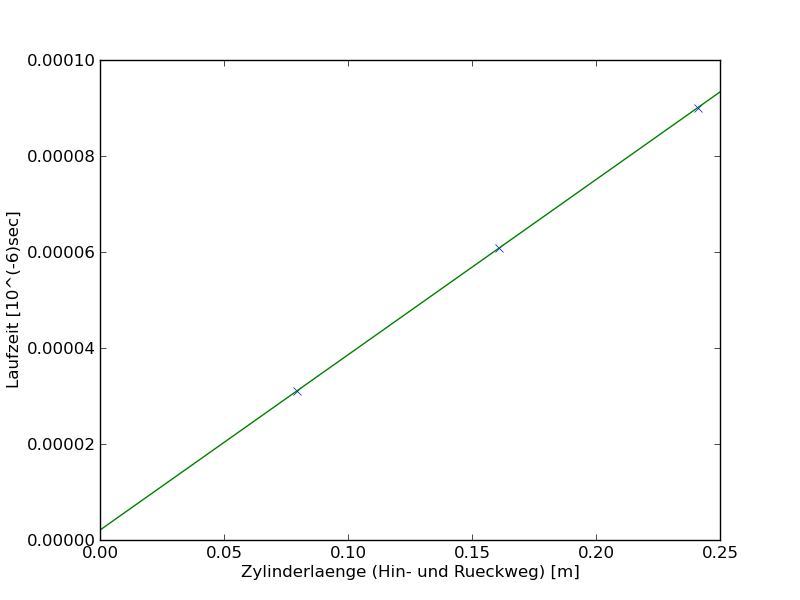
\includegraphics[width=12cm]{Fig1.png}
\caption{Plot für 1 MHz}
\label{fig1}
\end{figure}
\newpage
\begin{figure}[h]
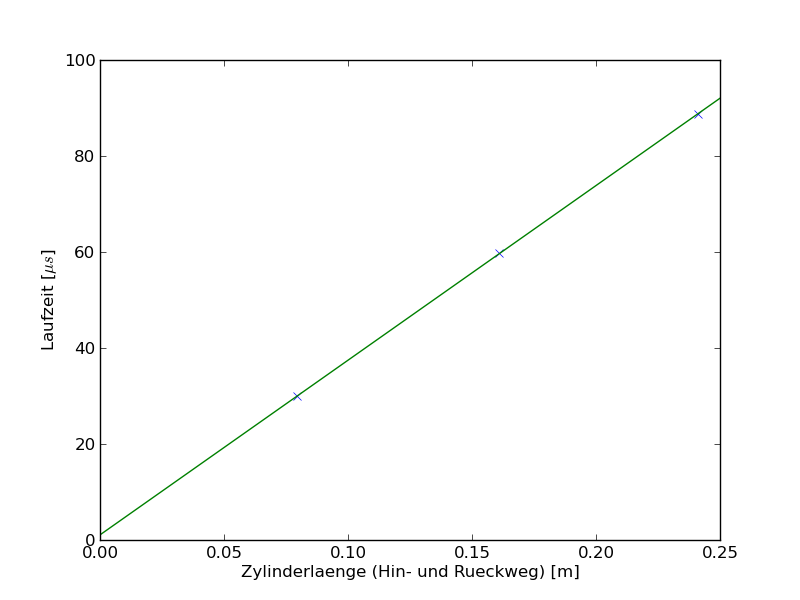
\includegraphics[width=12cm]{Fig2.png}
\caption{Plot für 2 MHz}
\label{fig2}
\end{figure}
\newpage
\begin{figure}[h]
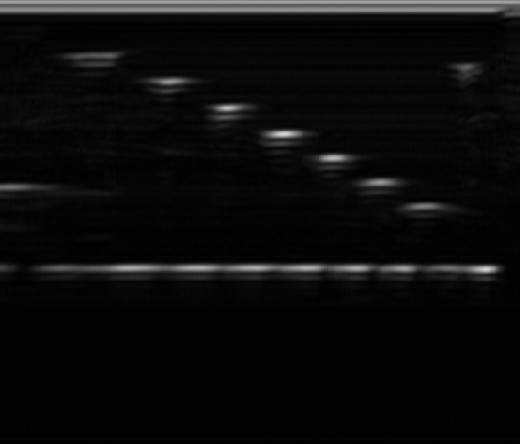
\includegraphics[width=12cm]{bscan1.jpg}
\caption{B-Scan des Acrylblocks}
\label{fig3}
\end{figure}
\newpage
\begin{figure}[h]
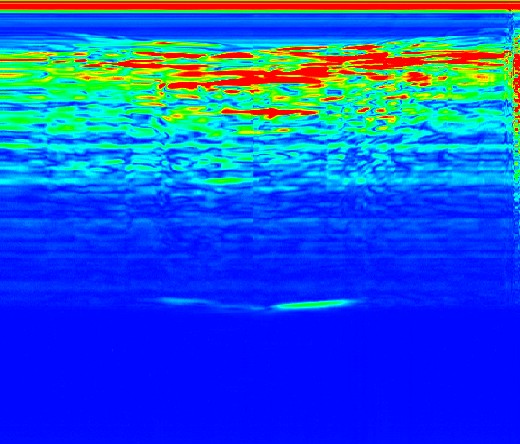
\includegraphics[width=12cm]{bscan2.jpg}
\caption{B-Scan des Auges}
\label{fig4}
\end{figure}
\end{document}
